%%%%%%%%%%%%%%%%%%%%%%%%%%%%%%%%%%%%%%%%%
% University/School Laboratory Report
% LaTeX Template
% Version 3.1 (25/3/14)
%
% This template has been downloaded from:
% http://www.LaTeXTemplates.com
%
% Original author:
% Linux and Unix Users Group at Virginia Tech Wiki 
% (https://vtluug.org/wiki/Example_LaTeX_chem_lab_report)
%
% License:
% CC BY-NC-SA 3.0 (http://creativecommons.org/licenses/by-nc-sa/3.0/)
%
%%%%%%%%%%%%%%%%%%%%%%%%%%%%%%%%%%%%%%%%%

%----------------------------------------------------------------------------------------
%	PACKAGES AND DOCUMENT CONFIGURATIONS
%----------------------------------------------------------------------------------------

\documentclass{article}

\usepackage[version=3]{mhchem} % Package for chemical equation typesetting
\usepackage{siunitx} % Provides the \SI{}{} and \si{} command for typesetting SI units
\usepackage{graphicx, xcolor} % Required for the inclusion of images
\usepackage{natbib} % Required to change bibliography style to APA
\usepackage{amsmath} % Required for some math elements 
\usepackage{svg} % .svg support
\usepackage[nolist]{acronym}
\usepackage{minted}
\definecolor{bg}{rgb}{0.95,0.95,0.95}

\graphicspath{{img/}}

\setlength\parindent{0pt} % Removes all indentation from paragraphs

\renewcommand{\labelenumi}{\alph{enumi}.} % Make numbering in the enumerate environment by letter rather than number (e.g. section 6)

%\usepackage{times} % Uncomment to use the Times New Roman font

%----------------------------------------------------------------------------------------
%	DOCUMENT INFORMATION
%----------------------------------------------------------------------------------------

\title{Projekt: Mobilfunk und Singalverabreitung} % Title

\author{Lukas Becker, Tobias Frahm} % Author name

\date{\today} % Date for the report

\begin{document}

\maketitle % Insert the title, author and date

\begin{center}
\begin{tabular}{l r}
Date Performed: & \today \\ % Date the experiment was performed
Partners: & Lukas Becker, Tobias Frahm \\ % Partner names
Instructor: & Prof. Dr. Sauvergerd \\% Instructor/supervisor
University: & University of Applied Science 
\end{tabular}
\end{center}

\begin{acronym}
    \acro{CPFSK}{Continus Phase Frequency Shift Keying}
\end{acronym}

% If you wish to include an abstract, uncomment the lines below
% \begin{abstract}
% Abstract text
% \end{abstract}

%----------------------------------------------------------------------------------------
%	SECTION 1
%----------------------------------------------------------------------------------------

\section{Projektbeschreibung und Ziel des Projektes}

In diesem Projekt wird eine \ac{CPFSK} Demodulation von Wetterdaten 
(Seewetterbericht des  Senders  Pinneberg  auf  Kurzwelle)  in  Echtzeit  durchgeführt. 
Diese  \ac{CPFSK} Demodulation  wird  in  Form  eines  \textit{Software  Radios}  auf  einem  
Digitalen Signalprozessor (DSP) implementiert. 

Die \ac{CPFSK}-kodierten Wetterdaten werden mit einer Draht-Antenne im Frequenzebereich
$10.1Mhz$ bis $11.1MHz$ empfangen und verstärkt. Bei dem so empfangenem Signal handelt es sich um 
\ac{CPFSK}-Modulierte Seewetterdaten. Ziel das Projektes ist es, zunächst in Matlab ein Modell zu erstellen, welches
in der Lage ist, die \ac{CPFSK} modulierten Seewetterdaten zu decodieren und diese auszugeben. 
Für das Matlab Modell wird hierfür zunächst ein \ac{CPFSK}-Signal in Matlab erzeugt um die ersten 
Schritte durchzuführen. Später in der Simulation kann hier auf ein Zeitbegrenztes Signal 
als Grundlage für das Matlab Modell genutzt zurückgegriffen werden. 
Sobald das Matlab Modell steht, wird die Simulation in C-Code überführt und anschließend 
auf einem DSP implementiert.

\section{Signalfluss Empfänger}

Abb.~\ref{fig:signal} zeigt den Aufbau des Softwareradios. Das $~11MhZ$ Signal wird empfangen, es findet eine erste Unterabtastung durch den ADC auf dem DSP statt.
Hierbei wird das Band auf ca. $2Mhz$ geschmälter. Das erste Filter, ein FIR-Polyphasen Bandpassfilter, Kapitel~\ref{sec:FIR}, mischt das Signal ein weiteres mal durch unterabtastung in einen Frequnzbereich
von wenigen kilo Herz. In dem so runtergemischten Band tritt nun entwederdie Mark (logisch 1), oder die Space (logisch 0) auf. Um hier differenzieren zu können,
muss können unterschiedliche methoden Angewandt werden, in dieser Arbeit wurde zunächst ein Ansatz über einen Hilberfilter, Kapitel~\ref{sec:hilbert}, verfolgt. Später hat sich jedoch das Kammfilter
als sinnvollere Alternative herausgestellt. Das Kammfilter in Kapitel~\ref{sec:comb} sorgt dafür, dass die Frequenzen deutlich von einander zu differenzierne sind. Sobald das Signal durch das Kammfilter
aufbereitet ist, kann die Demodulation durch einen FM-Verzögerungs Demodulator \ref{sec:fm-demod} mit anschließender Decodierung erfolgen.

\begin{figure}[!h]
    \centering
    \def\svgscale{0.5}
    \def\svgwidth{\columnwidth}
    \input{img/signal.pdf_tex}
    \caption{Durch den ADC findet direkt beim Empfang eine Unterabtastung statt. Durch eine weitere Unterabtastung im Bandpass, wird das Signal in das Basisband verschoben.
    Anschließen durch das Kammfilter für die Demodulation mit anschließender Decocdierung aufbereitet und auf dem Hyperterminal angezeigt.}
    \label{fig:signal}
\end{figure}

\section{FIR-Polyphasen Bandpass}\label{sec:FIR}
Das FIR-Polyphasen Bandpassfilter unterabtastet die 2MHz Signal ein weiteres mal durch eine Dezimationsstufe und mischt 
das Nutzsignal ins Basisband. Zunächst wird hierfür das FIR-Bandpassfilter in Matlab ausgelegt.
Anschließend werden die in Matlab erzeugten Koeffizienten aufgeteilt in 527 dezimationsstufen und in eine C-Datei geschrieben.
und später in der C-Implementierung verwendet. 

\subsection{Theorie}
In dem $~2MHz$-Signal befindet sich das eigentliche Nutzsignal $\frac{1MHz}{5kHz}$-Mal, um hier die beiden Frequenzen für $w_{mark}$ und $w_{space}$
aus einem der $5kHz$ Bänder herrauszufiltern, wird ein FIR-Bandpass mit Dezimationsstufe eingesetzt. Mit der Festgelegten Abtastfrequenz des ADC von $fA = 2,0192MHz$,
liegt der erste Träger bei $f_T \approx 4kHz$. Beachtet man nun das $\varDelta f = 742Hz$ breit ist, muss das FIR-Bandpassfilter mindestens ein Band von
$f_T \pm \frac{\varDelta f}{2}$ passieren lassen. Daraus ergibt sich ein notwendiger druchlassbereich von $B_{FIR} > 742Hz$. 
Sinnvolle Grenzen ergeben sich dann bei $f_u = 3800Hz$ und $f_o = 4800Hz$.


\subsection{Matlab}
Zu Auslegung des FIR Filters in Matlab lst.~\ref{codeM:FIRBP}, müssen zuächst die Grenz- und Stopfrequenzen Festgelegt werden.
Es ergeben sich $f_u = 3800Hz$ und $f_o = 4800Hz$, die Stopfrequenzen $f_{uStop} = f_u - 1500$ und $f_{oStop} = f_o + 1500$.
Bei den Stopfrequenzen gilt es Abzuwägen, umso steiler das Filter, desto mehr Koeffizienten, desto mehr Rechenzeit wird später in C
benötigt.
Der Amplitudengang des Filters, siehe Abb.~\ref{fig:fir_ampli}, zeigt das gewünschte Verhalten. Es werden $2056$ Koeffizienten benötigt.


\begin{figure}[!h]
    \label{fig:fir_ampli}
    \centering
    \def\svgscale{0.3}
    \def\svgwidth{\columnwidth}
    \input{img/FIR_BP.pdf_tex}
    \caption{FIR-Bandpassfilter Amplitudengang. Das FIR Filter benötigt 2056 Koeffizienten.}
\end{figure}
\begin{listing}\label{codeM:FIRBP}
    \caption{FIR Filter in Matlab}
    \begin{minted}[linenos, bgcolor=bg]{c}
function [outputArg1, outputArg2, outputArg3] = 
        band(low, high, inputSig, sample_rate)
%FIR Bandpass
%
rp = 3; 
rs = 40;
dev = [(10^(rp/20)-1)/(10^(rp/20)+1) 10^(-rs/20)]; 
low_stop = low - 1500;
high_stop = high + 1500;
[N_FIR,fo,mo,w] = firpmord([low_stop low high high_stop], 
                        [0 1 0], [0.05, 0.01, 0.05], sample_rate);
fprintf("N_FIR = %d\n", N_FIR);
coeff = firpm(N_FIR,fo,mo,w);

freqz(coeff,1, 200000, sample_rate)

xb = filter(coeff, 1, inputSig);
outputArg1 = xb;
outputArg2 = coeff;
outputArg3 = fo;
end
    \end{minted}
\end{listing}
\subsection{C}
In der C-Implementierung wird in der endgültigen Version mit dem Datentyp \textit{short} gearbeitet. 
Dies trägt zu einer besseren performance auf dem DSP bei.
Die Koeffizienten des FIR-Filters werden in $527$ \textit{const short} Arrays der Größe 4 aufgeteilt, siehe \ref{codeC:dezimation},
und in den FIR Filter übergeben. Es wird Sample für Sample eingelesen, dezimert und durch die Filterroutine verarbeitet lst.~\ref{codeC:FIR}.
\begin{listing}\label{codeC:dezimation}
    \caption{Beisphafte Polyphase in C, die Koeefizienten}
    \begin{minted}[linenos, bgcolor=bg]{c}
const short FIR_BANDPASS_1[4] = {1304, 22, 186, -8,};
    \end{minted}
\end{listing}


\begin{listing}\label{codeC:FIR}
    \caption{FIR-Polyphasenbandpass Implementierung in C}
    \begin{minted}[linenos, bgcolor=bg]{c}
short FIR_filter_sc(short FIR_delays[], const short FIR_coe[], 
        short int N_delays, short x_n, int shift) {
    short i, y;
    int FIR_accu32 = 0;
    // read input sample from ADC
    FIR_delays[N_delays-1] = x_n;	 
    // clear accu
    FIR_accu32	= 0;
    // FIR filter routine				
    for( i = 0 ; i < N_delays ; i++ )		
        FIR_accu32 += FIR_delays[N_delays-1-i] * FIR_coe[i];
    
    for( i = 1 ; i < N_delays ; i++ )				
        FIR_delays[i-1] = FIR_delays[i];

    y = (short) (FIR_accu32 >> shift);
    return y;
}
    \end{minted}
\end{listing}

\section{Hilbert Transformator}\label{sec:hilbert}
Der Hibert Transformator wandelt ein reeles Zeitsignal $x(t)$ in ein analytisches Signal $x_+(t)$ um.
Dies wird benötigt um das Signal anschlieend mit dem FM-Verzögerungs Demodulator, beschrieben in Kapitel \ref{sec:fm-demod}, zu demodulieren.
Mit $\mathcal{H}(x(t))$, der Hiltert Transformierten ergibt sich dies wie folgt:

$$ 
x_+(t) = x(t) + j \mathcal{H}(x(t))
$$

Wobei $y(t) = \mathcal{H}(x(t))$ sich mit mit $Y(f) = X(f) \cdot -j sign(f)$ berechnen lässt.
Wird dieses analytische Signal jedoch dem FM-Verzögerungs Demodulator übergeben, ist aufgrund des 
geringen Frequenzhubs $\varDelta f$ eine eindeutige Demodulation jedoch nicht möglich. Der Abstand zwischen beiden Signalen ist so gering, dass sich die 
Frequenzanteile von $w_{mark}$ und $w_{space}$ teilweise überlappen. Daher wird
dieser Ansatz auch nicht weiter verfolgt.


\section{Komplexes Kammfilter}\label{sec:comb}
Eine Alternative zu dem in Kapitel~\ref{sec:hilbert} beschriebenen Hilber Transformator ist ein Kammfilter.
Um die Frequenzen besser von einander differenziern zu können, wird ein Kammfilter genutzt. Dieser kann durch eine Anzahl $N$ Verzögerer realisiert werden.
Ziel in der Auslegung des Kammfilters ist es, die Nullstellen so zu legen, dass entweder $w_{mark}$ oder $w_{space}$ des Nutzsignals im positiven Frequenzbereich
gedämpft wird, und das jeweils andere $w$ im negativen Bereich. Zunächst wird das Filter dafürso Ausgelegt, das der Abstand zwischen
Nullstelle und Hochpunkt in der Filterübertragungsfunktion ca. dem Frequenzhub $\varDelta f$ entsprich, anschließend muss es so Verschoben werden, dass die Nullstellen wie beschrieben auf dem
gewünschten $w_{mark/space}$ liegen.
So wird der Frequenzunterschied zwischen den beiden Frequenzen von $\varDelta f$ auf $2\cdot fA$ angehoben.
Die Frequenzen sind damit deutlich unterscheidbar und können im nächsten Schritt, der Demodulation eindeutig zugeordnet werden. 

\subsection{Theorie}


Ausgehend von der Übertragnungsfunktion 
$$H(z) = 1 + z^{-N}$$ 
mit 
$$ z = e^{j\omega} $$
ergibt sich

$$H(j\omega) = 1 + e^{-j\omega N}$$

und dem ausklammern von $ e^{-j \frac{\omega N}{2}}$:
$$
H(e^{j\omega}) = e^{-j \frac{\omega N}{2}} \cdot (e^{-j \frac{\omega N}{2}} + e^{j \frac{\omega N}{2}})
$$

$e^{-j \frac{\omega N}{2}} \neq 0$ daher wird nur $(e^{-j \frac{\omega N}{2}} + e^{j \frac{\omega N}{2}})$ weiter betrachtet

Es gilt:
$$
(e^{-j \frac{\omega N}{2}} + e^{j \frac{\omega N}{2}}) = 2  cos(\frac{\omega N}{2})
$$
Zur bestimmung der Nullstellen, Argument des Cosinus betrachten.

Allg.: $0 = cos(\frac{\pi}{2} + k\pi)$
$$
\frac{w_0 N}{2} = \frac{\pi}{2} + k\pi
$$

$$
<=> w_0 = \frac{2\pi k + \pi}{N}
$$
mit $k = 0$, $w_0 = 2\pi \cdot \frac{f}{fA}$ und nach $N$ Aufgelöst, ergibt sich:

$$
<=> N = \frac{\pi}{2\pi \frac{f}{fA}}
$$
eingesetzt:

$$
N = \lfloor \frac{\pi}{2\pi \frac{450Hz}{3832Hz}}\rfloor = 4
$$

Der Faktor N bestimmt die Anzahl der benötigten Verzögerer, damit $\omega_0$ im idealfall genau so auf $\omega_{mark}$ oder $\omega_{space}$ liegen dass eine der beiden 
Frequenzen im positiven Frequenzbereich gedämpft wird und die andere im Negativen. In diesem Fall liefert $N = 4$ das gewünschte Ergebnis, siehe Abb.~\ref{fig:comb}, Latexcode \ref{codeM:comb}

\subsection{Matlab}
In Matlab wird das Filter überprüft, Implementiert wird das Filter mithilfe von 4 Verzögerern.
Dafür wird in Matlab ein mit $N$-Nullen gefülltes Array verwendet. In Abb.~\ref{fig:comb} ist zu sehen,
dass die Nullstellen des Kammfilter sehr gut auf den jeweileigen Frequenzen $- w_{mark}$ und $w_{space}$ liegen.

\begin{listing}
    \label{codeM:comb}
    \caption{In Matlab wird Überprüft ob die Berechnung des $N$ korrekt sind, indem das Filter mit den Frequenzen
    $w_{mark}$ und $w_{space}$ geplottet wird, siehe Abb.~\ref{fig:comb}. Es wird kontrolliert ob die Nullstellen in den richten Punkten auf der Frequenzachse liegen.}
\begin{minted}[linenos, bgcolor=bg]{matlab}
    N = 4
    fA_green = 3832;
    freq_comb = (-fA_green:fA_green)/fA_green;
    
    H_comb = freqz([zeros(1,N), 1], 1, 2*pi*freq_comb)
                +i*freqz(1,1,2*pi*freq_comb);
    
    figure(4);
    plot(freq_comb, abs(H_comb), 'b-')
    hold on;
    stem(-732/fA_green, 2, 'k');
    stem(-1187/fA_green, 2, 'r');
    stem(732/fA_green, 2, 'k');
    stem(1187/fA_green, 2, 'r');
    grid on
    hold off;
    xlabel(['normierte Frequenz'])
    ylabel(['Amplitude'])
    title('Amplitudengang Kammfilter');
\end{minted}
\end{listing}

\begin{figure}[!h]
    \label{fig:comb}
    \centering
    \def\svgscale{0.3}
    \def\svgwidth{0.8\columnwidth}
    \input{img/comb_6n.pdf_tex}
    \caption{Kammfiter mit den deiden Frequenzen $\omega_{mark}$ und $\omega_{space}$, das Kammfilter lässt jeweils eine der beiden Frequenzen passieren.}
\end{figure}
\subsection{C}
Für die C-Implementierung, siehe \ref{codeC:comb}, wird jedes eingabe Sample um $N = 4$ verzögert.
Die Verzögerung wird über ein Buffer Array der Länge $N$ realisiert:
\begin{listing}\label{codeC:comb}
    \caption{C-Implementierung des Kammfilters mithilfe eines Verzögerer Buffers}
    \begin{minted}[linenos, bgcolor=bg]{c}
        short delayed_sample = 0;
        short cnt = 0;
        short *delay_iter = NULL;
        short delay_line[4];
        short *rotating_rw = delay_line;
 
        static void process_comb_and_demod() {
            // Comb filter
            I_sig = dec_out_short + 175 * delayed_sample;
            Q_sig = 984 * delayed_sample;
            ....
        }

        static void output_sample() {
            dec_out_short = dec_out >> 5;

            // Delayline counter overflow management
            if (rotating_rw == delay_line + 4)
                rotating_rw = delay_line;
            
            // Rotating delayed sample storage
            delayed_sample = *rotating_rw;
            *rotating_rw = dec_out_short;
            rotating_rw += 1;

            cnt++;
        }
    \end{minted}
\end{listing}

\section{FM-Verzögerungsdemoulator} \label{sec:fm-demod}
Der FM-Verzögerungsdemoulator wird im Worksheet 2 des Projekts Behandelt. 
Der FM-Verzögerungsdemoulator soll das CPFSK-modulierte Signal demodulieren und eine Rechteckfolge ausgeben.
Der eigentliche Ansatz aus Worksheet zwei mit einem abschließendem sinus als nicht liniarer Verstärker funktioniert idR nicht, 
da die Frequenzen von $w_{mark}$ und $w_{space}$ aufgrund der Symmetrie des Sinus ($sin(f) = sin(-f)$) nicht mehr von einander zu Unterscheiden sind.

\textit{Warum gehts denn doch? Was machen wir anders?}
\subsection{Matlab}

\subsection{C}

\section{Decodierung}

Die Decodierung liest die $D = \{0,1\}$ Bitweise ein und schiebt diese in einen Buffer. 
Die Symbolfrequenz von $50Hz$ bestimmt die Abtastrate des Decodierers. Da bei dem Start/Stop-Bit um das
halbe Bit der Stop-Sequenz erkennen zu können liegt hier folgender Ansatz zugrunde:

$$
f_{decode} = \lfloor fA * \frac{1}{f_{symbol} \cdot 2}\rfloor 
$$
eingesetzt
$$
f_{decode} = \lfloor 3832Hz * \frac{1}{50Hz\cdot 2}\rfloor = 38
$$
Für die Implementierung wird im C-Code der Aufruf druch eine einfach $IF$ und eine Zählvariabel
gesteuert. Der Decodierer, siehe \ref{codeC:decode}, schiebt Bit für Bit durch einen Buffer, liegt
die Start/Stop Sequenz $0x001F$ in dem Buffer, werden die nächsten $10$ Bits, als Bits eines Buchstaben interpretiert.
Jeder Buchstabe wird durch 5 Bits repräsentiert, in \ref{codeC:decode} ab Zeile 20 um die hälfte komprimiert.
Das daraus erzeugt Ergebnis, repräsentiert den Index einer LookUp Table für den entsprechen Buchstaben.

\begin{listing}\label{codeC:decode}
    \caption{C-Implementierung: Funktion des Decodierers}
    \begin{minted}[linenos, bgcolor=bg]{c}
void decode(unsigned short bit) {

    if (!current_lut) 
        current_lut = lookup_char;

    buffer = buffer << 1;
    buffer = buffer | bit;
    startstop = buffer & 0x001F;

    if (startstop_holdoff > 0) // Underflow protection
        startstop_holdoff -= 1;

    if (startstop == STOP_SEQUENCE && startstop_holdoff == 0) {
        startstop_holdoff = 11;
        // Shift over the start and stop section
        // and mask the 10 message bits
        index_pre = (buffer >> 5) & 0x03FF; 
        // Compress bit stream to half its size
        // Turn this 1 1 1 1 0 0 1 1 0 0 into 1 1 0 1 1
        real_index = (((index_pre >> 0) & 0x0001) << 4) 
                | (((index_pre >> 2) & 0x0001) << 3) 
                | (((index_pre >> 4) & 0x0001) << 2) 
                | (((index_pre >> 6) & 0x0001) << 1) 
                | (((index_pre >> 8) & 0x0001) << 0);

        if (real_index == SWITCH_TO_CHAR) {
            // Change to characters
            current_lut = lookup_char;
        } else if (real_index == SWITCH_TO_NUM) {
            // Change to numbers
            current_lut = lookup_num;
        } else {
#ifdef USE_MSVC_ANSI_C_SIM
            // Everything else is a valid character
            printf(" >> %c <<\n",current_lut[real_index-1]); 
#endif
        }
    }
}
    \end{minted}
\end{listing}





--------------------------------------------------------------------------------------------------

\section{Simulation: Matlab}
In dem folgenden Kapitel wird zunächst ein Rechteckimpuls auf eine Trägerfrequenze mithilfe der \ac{CPFSK} moduliert.


\subsection{CPFSK Modulation}
Die \ac{CPFSK} Modulation ist eine Methode um digitale Signale mithilfe einer Trägerfrequenze analog zu Übertragen.
Bei der \ac{CPFSK} Modulation handelt es sich um eine Frequenzmodulation ohne Sprünge im Phasenübergang. In Abb.~\ref{fsk}
ist im oberen Bereich das binäre Signale, im mittleren Bild die Trägerfrequenze und unten das binäre Signal auf die Trägerfrequenze
moduliert zu sehen. Der Phasenübergäng ohne Sprung ist notwendig, da Sprünge ein theoretisch unendliches breites Band benötigen
somit die Nachbarkanäle stören würde.
\begin{figure}[!h]
    \centering
    \def\svgscale{0.3}
    \def\svgwidth{\columnwidth}
    \input{img/fsk.pdf_tex}
    \caption{Beispielhaftes \ac{CPFSK} moduliertes Trägersignal einer binären 
    Information. Die Phasenübergänge sind ohne Sprung. Quelle:~\cite{wiki:fsk}}
    \label{fsk}
\end{figure}
\subsection{Rechteckimpuls $d(i)$}\label{sec:rechteck}
Mit Angabe der Symboldauer $T = 20ms$ lässt sich auf die minimale Abtastfrequenz nach Nyquist-Shannon schließen.
Die minimale Abtastfrequenz $f_A$ muss mehr als doppelt so groß wie die höhste abzutastende Frequenz sein.

Aus
\begin{center}
 $
f_A > 2*f_{max}
$
\end{center}

mit 
\begin{center} $f_{max} = \frac{1}{T_{max}} ; T_{max} = T = 20ms$  \end{center}

ergibt sich

\begin{center}
$
f_A > 2*\frac{1}{T}
$
\end{center}

Eingesetzt:
\begin{center}
$f_A > 2*\frac{1}{20ms}$
\end{center}
\begin{center}
$f_A > 100Hz$   
\end{center}
\begin{figure}[!h]
    \centering
    \def\svgscale{0.3}
    \def\svgwidth{\columnwidth}
    \input{img/rechteck.pdf_tex}
    \caption{Recheckimpuls zur \ac{CPFSK} Simulation in Matlab}
\end{figure}

\subsection{Anfangsphase $\phi(iT)$}

Gegeben ist die ein Integrator (IIR Filter 1.Ordnung) mit der Übertragnungsfunktion:
$$
H_I(z)=\frac{z^{-1}}{1-z^{-1}}
$$
Dieser kann hier anstelle der Summenbildung der komplexen Einhüllenden eingesetzt werden, 
da die Integration einer Aufsummierung diskreter Flächenelemte unter der Kurve entspricht.

\begin{figure}[!h]
    \centering
    \def\svgscale{0.3}
    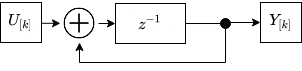
\includegraphics{img/sig_IIR.png}
    \caption{Signalflussdiagramm des Integrators 1.Ordnung}
\end{figure}

\subsection{CPFSK Signal}
Das in Abschnitt~\ref{sec:rechteck} generierte Reckecksignal wird nun CPFSK Modeliert.
Dafür wir die Formel aus Worksheet 1 verwendet:

$$CPFSK_{sig} = amp \cdot  sin(2  pi \cdot f_T \cdot n \cdot T_A + 2 pi \cdot \varDelta{F} \cdot \frac{\phi (iT)}{f_A} + \varphi{0}) $$

Zur bestimmung des Spektrums des Signals, wird in Matlab FFT verwendet.
\begin{figure}[!h]
    \centering
    \def\svgscale{0.3}
    \def\svgwidth{\columnwidth}
    \input{img/spektrum.pdf_tex}
    \caption{Betragspektrum des CPFSK-Modulierten Rechteckimpulses.}
\end{figure}
Bei einem $\varDelta(F) = 225Hz$ wird hier eine Bandbreite von ca. $B > 450Hz = 2\cdot \varDelta(F) $ erwartet.

Zur Bandbreitenbestimmung wird das Parsevalsche Theorem genutz, die Bandbreite des CPFSK Signals ist derjenige Bereich,
in den 99\% der Signalenergie von $0...\frac{f_A}{2}$ Fallen. Es ergibt sich hierbei eine Bandbreite von $536Hz$

$$
\sum_{n = 0}^{N - 1}\left\lvert x(n)^2\right\rvert =  \frac{1}{N} \sum_{k = 1}^{N-1}  \left\lvert X(k)^2\right\rvert 
$$

\begin{minted}{matlab}
% Die Bandbreite wird durch den Breich beschrieben, in den 99% der
% Signalenergie fallen.

total_power = 0;
current_power = 0;
idx = 0;
idx_max = round(length(spectrum_sig)/2);
idx_start = idx_max/2; % fA/4

for i = 1:length(spectrum_sig)/2 - 1
    total_power = total_power + abs(spectrum_sig(i))^2 / length(spectrum_sig);
end

N = length(spectrum_sig);

while current_power/total_power < 0.99
    current_power = current_power + abs(spectrum_sig(idx_start - idx))^2 / N;
    current_power = current_power + abs(spectrum_sig(idx_start + idx))^2 / N;
    idx = idx + 1;
end

fprintf("Bandbreite: %dHz\n", ((idx_start + idx) - (idx_start - idx)))
\end{minted}

Das Weglassen der Start- und Stoppbits spielt bei der bestimmung der Bandbreite keine rolle.
Es werden nur binäre Daten übertragen $D = \{0, 1\}$. die Frequenzen $ f_1 = f_T \pm \varDelta F $ repräsentieren. 
Da auch die Start/Stopbits durch $D$ dargestellt werden, würde sich hier im Frequenzbereich
nur eine veränderung im maximum der Amplitude ergeben, die repräsentierenden Frequenzen selbst bleiben unverändert.



% ---------------------------------------------------------------------------
%	BIBLIOGRAPHY
%----------------------------------------------------------------------------------------

\bibliographystyle{apalike}
\bibliography{lib}

%----------------------------------------------------------------------------------------


\end{document}